\chapter{Related Work}
\label{ch:related}

\section{Classical Train Longitudinal Dynamics and Simulation}

Longitudinal train dynamics (LTD) is the study of the physical interactions within a connected train body comprised of multiple linked masses, henceforth referred to as a \textit{consist}. Classical longitudinal train dynamics is defined as the motion of rolling stock vehicles in the longitudinal dimension of the track, ignoring lateral or vertical forces in most cases. The motion of the whole train as well as the individual motions of each vehicle are accounted for in this schema \cite{Cole2006HandbookLTD}.

Early attempts at LTD study treated a train as a continuous elastic rod with a traction force applied at one end, and enabled the study of longitudinal vibration phenomena. This later progressed to discretized mass-spring chains. Early models such as these generally ignored discontinuities, such as those arising from coupler slack, which enabled closed form solutions that required no numerical solver. Nonlinearities were identified early, such as draft gear behavior, but could not be simulated with the level of computing power at the time \cite{Wu2016OverviewLTD}. 

\subsection{Modeling Abstractions and Levels of Fidelity}

LTD can be framed as layered abstractions with increasing levels of complexity. At the greatest order-reduction level, LTD can be modeled as point mass or a single-body train model. This level of complexity can be useful for modeling energy usage or scheduling, but is highly limited in the observability of the system, i.e. many variables are unaccounted for. At the next level of abstraction, the consist can be modeled as a multi-mass system, where each vehicle is accounted for as a rigid body with one longitudinal degree of freedom. Masses are connected with modeled couplers and draft gears, which introduce nonlinear interactions. Beyond this, we can extend the DOF of the model to account for motions in the remaining spatial dimensions, which allows for observability track curve effects, in train instabilities, and even derailment scenarios; such models are formulated using the general multibody dynamics machinery of constrained rigid and flexible bodies \cite{shabana_multibody}. This scale of modeling naturally trades speed for fidelity, as computation of so many parameters is highly expensive, but the high fidelity is necessary for some analyses \cite{Wu2016OverviewLTD}.

\subsection{Computational Schemes and Numerical Challenges}

The standard computation schema for LTD treats the problem as an repeated evaluation of all force elements followed by state propagation \cite{Wu2018ComputingSchemesLTD}. In general, a simulator first identifies force elements (propulsion resistance, curving resistance, grade components, gravity, traction forces, dynamic brake forces, air brake forces, and coupler forces). Then, the system computes each element from the inputs (time, vehicle velocities, accelerations, and vehicle locations). Finally, velocities and positions are updated through a numerical solver. The clear modularity of this computing system allows for addition or replacement of new computing models, such as replacing a module with a learned surrogate model. 

The critical difficulty with computing LTD is with the vehicle connection systems, specifically the couplers, draft gears, and drawbars. Friction draft gears exhibit extreme nonlinearities, including hysteresis and stick-slip) that are hard to both model and numerically solve \cite{Wu2016OverviewLTD}. The coupler force calculation accounted for approximately $65\%$ of the computing time in the study described in \cite{Wu2018ComputingSchemesLTD}. That the cost concentrates so heavily in one force element is what makes a surrogate attractive here: the expensive part of the calculation is also the nonlinear, discontinuous part, and it is the part a learned model is best placed to absorb while the remaining force terms stay analytic. 

\subsection{Benchmarking, Applications, and Limitations}

LTD has historically lacked standardized procedures for benchmarking LTD simulators, which limits objective comparison of tools developed by different institutions. Spiryagin et. al. introduced an international benchmarking initiative to define a mutual set of input scenarios, operating conditions, and necessary outputs to compare efficacy of various simulators \cite{Spiryagin2017BenchmarkQuestions}. The benchmarking initiative was motivated by the fact that most LTD simulation tools have evolved independently as in-house software for the many institutions that use them. This resulted in limited to no transparency in terms of numerical methods, assumptions, and performance. Participating simulators used identical train configurations, commands for traction and braking, and track profiles. Outputs were measured in high temporal resolution to enable detailed comparison. This work provides an indispensable reference point for evaluating simulation fidelity and computational performance. The work further motivates the need for reproducible, scenario-based evaluation systems. 

The applications of LTD, especially rapidly evaluated scenarios, is further highlighted in the Wu-Spiryagin-Cole paper. Driving advisory systems are integrated computation engines which advise locomotive operators to take actions based on instrumented vehicle data. These systems require real time evaluation of LTD outputs. Furthermore, energy consumption calculations can be evaluated from a simulator with observable traction/braking forces and speed/distance signals. Such energy estimates are only as accurate as the model's treatment of the interactions that are hardest to capture, chiefly those at the couplers. Fatigue and safety analyses depend on time-domain histories of dynamic interactions, which can be invaluable for risk assessment. 

% Table: LTD simulation tools comparison
% Requires: textcomp (in preamble, for \texttrademark)

\begin{table*}[t]
\centering
\small
\caption{Representative longitudinal train dynamics (LTD) simulation tools}
\label{tab:ltd_tools_comparison}
\renewcommand{\arraystretch}{1.1}
\setlength{\tabcolsep}{3pt}
\begin{tabular}{@{}p{2.5cm}p{3.5cm}p{5.5cm}p{2.5cm}@{}}
\toprule
\textbf{Tool} & \textbf{Origin} & \textbf{Scope} & \textbf{Availability} \\
\midrule
\textbf{TrainDy} \cite{Cantone2008TrainDy} &
UIC-oriented (academic/industry consortium) &
Freight LTD for operations and safety analysis &
Specialized / consortium \\

\textbf{TOES\texttrademark} \cite{WheelRail2018TOES} &
Developed for AAR-member railroads &
Comprehensive train dynamics for operating scenarios &
Commercial / licensed \\

\textbf{TEDS} \cite{FRA2019TEDSProject,FRA2015TEDSValidation} &
U.S. FRA-sponsored (contractors) &
Safety/risk evaluation, incident investigation, operations LTD &
Publicly documented \\

\textbf{UM Train} \cite{UMTrainPlugin} &
Universal Mechanism suite &
Train longitudinal dynamics within multibody ecosystem &
Commercial \\

\textbf{TDEAS} \cite{Wei2014TDEAS} &
Developed in China (research/industry) &
LTD + energy analysis &
Research / institutional \\

\textbf{CRE-LTS} \cite{Spiryagin2017BenchmarkQuestions} &
Centre for Railway Engineering (CQU) &
Benchmarking-ready research LTD simulator &
Research / in-house \\
\bottomrule
\end{tabular}
\end{table*}

\vfill

\section{Data-Driven and Hybrid Modeling in Rail}

The computational expense and architectural complexity of high-fidelity rail models have motivated a growing body of work on data-driven and hybrid modeling approaches. These methods utilize machine learning for acceleration of classical simulations, estimation of unmeasured internal quantities, or enabling of real-time decision support. In general, models maintain an interpretable physics-based backbone where possible, but this line is blurred when more advanced "black-box" models are introduced. Existing efforts, in general, fall into three overlapping categories: surrogate replacement of expensive physics submodels, data-driven estimation of in-train forces from operational data, and surrogate modeling for optimization and fleet/network level decision-making.

\subsection{Surrogate Models for Accelerating Physics-Based Simulation}

One prominent line of research focuses on embedding learned surrogate components within classical multibody or finite-element-based simulation frameworks. Instead of replacing the entire physics model with a "black-box" technique, these approaches substitute the most computationally intensive or nonlinear subcomponents with data-driven approximations trained on simulation data. For example, Nie et al. train surrogate elements on finite-element outputs and substitute them for the corresponding mechanical elements inside a multibody vehicle dynamics simulation, coupling MATLAB/Simulink with SIMPACK; they report that a Legendre polynomial regression surrogate substantially reduces computing time without sacrificing accuracy \cite{nie_data_driven_dynamics}. Polynomial regression, Kriging, and other response-surface techniques are commonly employed in this setting, as they are highly interpretable and allow scientists and engineers to make grounded deductions.

More recent work has emphasized system integration of machine learning surrogates into digital twin architectures. In this schema, a full multibody dynamics (MBD) model is replaced by a neural network based surrogate and packaged using standardized interfaces such as the Functional Mock-up Interface (FMI). This enables deployment as a Functional Mock-up Unit (FMU) within larger co-simulation or decision-support environments \cite{zhou_surrogate_integration}. Zhou et al. report that a recurrent neural network surrogate evaluates a 5\,km track segment in roughly eight seconds, against approximately thirty minutes for the equivalent multibody simulation in SIMPACK, and they demonstrate a practical pipeline for continuous model deployment. However, this line of work remains primarily focused on reproducing nominal simulator behavior rather than modeling uncertainty or difficult component interactions.

\subsection{Data-Driven Estimation of In-Train Forces}

A second major branch of data-driven rail modeling targets the estimation of in-train forces, which are difficult to measure directly in operational freight and passenger trains. Leveraging the increasing availability of onboard telemetry, particularly from Automatic Train Operation (ATO) systems, several authors have proposed supervised learning approaches that map operational signals such as speed, acceleration, and control commands to coupler force estimates. Convolutional neural networks (CNN) augmented with causal structure and self-attention mechanisms have demonstrated accurate reproduction of simulator-derived force histories under typical operating conditions \cite{zhang_in_train_forces}.

Extensions of this concept incorporate multi-task learning and transfer learning to generalize force estimation across multiple couplers and train configurations. The In-trainNet framework, for example, first pre-trains a multi-task model that estimates forces at several couplers of one train configuration, then adapts that pre-trained representation to different configurations through transfer learning, substantially reducing the volume of training data each new configuration requires \cite{intrainnet}. While these approaches represent an important step toward scalable “virtual instrumentation” of in-train forces, they are generally trained on labeled data generated by longitudinal train simulators and are validated on limited scenario sets.

\subsection{Surrogate Modeling for Operations and Optimization}

Data-driven surrogates have also been employed to accelerate optimization problems in railway operations, transcending the low-level dynamics and force estimation problems and solving high-level, or even fleet level problems. In the paper from Liu et. al., surrogate models are used to approximate the evaluation of candidate rail schedules, significantly reducing the amount of expensive computation required during optimization \cite{liu_rescheduling_surrogate}. These methods search over multiple surrogates jointly and employ transfer learning, in this case to compensate for incomplete and imbalanced historical disruption data rather than for computational cost alone. Although effective in reducing computational burden, such surrogates are typically designed for specific operational contexts and rely on deterministic predictions of performance metrics for validation.

\subsection{Limitations of Existing Data-Driven and Hybrid Approaches}
\label{sec:rail_data_driven_limits}

Despite demonstrated success on several rail domains, existing data-driven and hybrid rail models exhibit several notable limitations. First, the majority of proposed surrogates are deterministic, providing point estimates without measures of predictive uncertainty. This limits their reliability when deployed outside the training distribution or when embedded within control and optimization loops where constraint violations can have significant consequences.

Second, generalization across operating schemes and consist configurations remains a persistent challenge. Force-estimation models of this kind are typically developed for a single coupler position within a single train configuration, so a separate model must be trained for each coupler and each consist of interest \cite{zhang_in_train_forces}. Subsequent work addresses this limitation directly through multi-task pre-training and transfer learning across configurations, but still requires configuration-specific adaptation data rather than generalizing to an arbitrary consist without retraining \cite{intrainnet}. These issues are exacerbated by the reliance on simulated labels, as discrepancies between simulation and real-world behavior can compound errors in purely data-driven mappings.

Finally, while hybrid surrogate approaches retain a physics-based structure, they are generally aimed at replication of nominal simulator outputs rather than modeling of epistemic uncertainty arising from unmodeled dynamics, parameter variability, or environmental disturbances. As a result, current surrogates offer limited robustness under distribution shift, constraining their applicability to safety-critical tasks such as energy-optimal control or real-time operational decision-making. Furthermore, the lack of baseline physical interpretability limits the industry adoption of new simulator technology, as rail engineers and scientists may be skeptical about a fully black-box prediction model (such as neural network).

\subsection{Implications for Structural Generalization}

Collectively, this body of work demonstrates that data-driven methods can accelerate railway simulation substantially, while also exposing a consistent structural limitation: each surrogate is tied to something particular. A model is trained for one coupler position, one consist configuration, one track segment, or one operational context, and a change in that quantity requires retraining or configuration-specific adaptation data. The generalization sought in this thesis is therefore not primarily statistical but structural. What is required is a model whose representation of a train does not encode a particular train, so that consist length becomes a property of the input rather than of the architecture. The remainder of this chapter reviews the two families of architecture that might plausibly supply that property.


\section{Transformers for Dynamical Systems and Spatiotemporal Forecasting}

Transformer architectures demonstrate strong candidacy for general purpose sequence modeling tasks. They have been increasingly adopted for dynamical systems modeling research and spatiotemporal forecasting. Transformers enable adaptive context aggregation over long temporal horizons by replacing recurrence with multi-head self attention. Unlike recurrent architectures, transformers do not impose a sequential dependency in their core computation. This intrinsic algorithmic feature allows transformers to be highly parallelizable during training. Transformers are particularly attractive for dynamical systems where future states often depend on long range temporal interactions, as trajectories can be represented as sequences of states or latent tokens \cite{vaswani2017attention}.

\subsection{Long-horizon Forecasting Transformers}

A major branch of work in transformers is focused on long horizon temporal forecasting. Standard self-attention scales quadratically with sequence length, which severely limits it's applicability to long-history prediction problems where fine-temporal resolution is necessary for accuracy. Informer addresses this problem by introducing ProbSparse attention, which identifies and attends to the most informative queries. This enables reduction in the computational cost for training in long horizon scenarios, but preserves enough necessary information to retain prediction accuracy. Compared to conventional models, Informer is capable of forecasting over substantially longer periods \cite{zhou2020informer}. 

Autoformer is an additional architecture proposed by Wu et. al. which is motivated by the observation that many real-world time series phenomena (such as energy demand, traffic flow, and economic trends) are dominated by two distinct patterns. These include a slowly varying yet long-term trend, and repeating or periodic behavior (seasonal). At great computational cost, a neural network could be used to discover these structures implicitly. Autoformer builds these phenomena directly into the model, where the input time series is first decomposed into trend and seasonal components to enable the model to address long term evolution and short term noise/fluctuations separately. Further, Autoformer replaces scaled dot-product attention with an auto-correlation mechanism that explicitly searches for repeating temporal patterns across various time windows. If recurrent structures are identified, they can be reused more efficiently. Thus, Autoformer improves prediction accuracy and stability for long time series systems by reducing the computational burden of learning every single interaction between time steps \cite{wu2021autoformer}.

Another promising architecture is the Temporal Fusion Transformer, which are designed for practical forecasting problems where predictions depend on many different types of information, not just a single time series data history. In applications, forecasting requires a combination of static attributes that do not change over time (such as system configuration or asset type), inputs that are known in advance (such as schedules, calendars, or planned control actions), and external variables that are observed over time but not controlled (such as weather or demand signals). Temporal fusion transformers partition these inputs instead of processing them all as a single, aggregate sequence. The model features mechanisms to determine which variables are the most relevant for prediction at each point in time. This structure allows TFT to generate multi-step forecasts while also providing interpretable information about which inputs most strongly influenced the predictions and when they were important, making the model more transparent and suitable for decision-support applications \cite{lim2019tft}. These properties make the model more transparent and interpretable, as compared to a black-box model.

\subsection{Neural Operators for PDE-governed Dynamics}

For spatiotemporal physical systems, forecasting can be cast as learning a solution operator mapping initial/boundary conditions (and coefficients/forcing) to future fields. Fourier Neural Operators (FNO) address forecasting and dynamical modeling problems from predicting individual timesteps to learning the governing function for how a system evolves. Instead of operating at specific values, FNO learns how information propagates across the entire spatial domain at once. As the name suggests, it does this by transforming the system state into the frequency domain, where long-term or broad patterns can be analyzed and computed much more efficiently. Within this new domain, the model applies global updates that resemble system-wide interactions rather than local point to point updates. As these learned updates are defined independently of any spatial configuration, the resulting model can be evaluated on finer or coarser spatial grids than those seen during training. This allows FNO based models to generalize across different spatial resolutions, making them well suited as fast, flexible surrogates for complex dynamical simulation \cite{li2021fno}.

Physics-informed neural operators (PINO) expand on operator-learning models by explicitly incorporating known physical laws into the training process. In many engineering or scientific systems, the governing equations for how the system evolves over time are at least partially known. PINO leverages this knowledge by penalizing violations of the underlying physical formulation (the differential equations governing the system) during training, rather than relying solely on error measurements from data. In practice, the model may be trained using available simulation or measurement data at a relatively coarse spatial or temporal resolution, while simultaneously evaluating how well predictions satisfy the governing physical equations at a finer resolution. The resulting model is a generalizable forecaster that respects known physical constraints. The framework allows for the creation of models even when data is limited or expensive to obtain \cite{li2021pino}.

Beyond representations that rely only on Fourier representations, Cao investigates how attention mechanisms (which were originally created to model sequences) can be used to directly learn the rules of evolution for dynamical systems \cite{cao2021choose}. The study compares Fourier-based representations, which emphasize global frequency patterns, with Galerkin-style representations, which are rooted in classical numerical methods that approximate solutions using weighted basis functions. In analyzing how self-attention interacts with these different representations, the work shows that no single formulation is universally optimal. The choice depends on the structure of the underlying system and the types of interactions that dominate its dynamic evolution. This perspective reframes operator learning as an architectural design problem, where decisions about how to represent space, enforce structure, and aggregate information are as important as the learning algorithm itself.

More recently, attention-based models have been adapted specifically for learning the evolution of systems governed by partial differential equations. In this line of work, Transformer-style architectures are reformulated to learn solution operators that map initial conditions, system parameters, and external inputs directly to future system states. As opposed to advancing the state forward step by step in time, the model learns a global input–output relationship that captures how the entire state evolves. The attention mechanism enables the model to aggregate information across spatial locations and time, allowing it to represent long-range interactions that are common in physical systems. Utilizing Transformer architectures within an operator-learning framework and evaluating them on canonical PDE benchmarks, this work demonstrates that attention-based models can serve as effective and general surrogates for complex spatiotemporal dynamics, further validating the use of Transformer-style mechanisms in scientific and engineering modeling contexts \cite{li2023transformerpde}.

\subsection{Implications for Train Dynamics and Spatiotemporal Decision Support}

These elements motivate hybrid modeling strategies for systems like train longitudinal dynamics where dynamics are structured (physics, constraints, conservation-like relationships) yet exhibit long-range dependencies (consist interactions, route profile memory, control plans). Forecasting-oriented Transformers (Informer/Autoformer/TFT) supply scalable mechanisms for long-horizon sequence prediction and covariate fusion \cite{zhou2020informer,wu2021autoformer,lim2019tft}, while neural-operator perspectives (FNO/PINO and attention-based operator learners) suggest a principled route to learning dynamics as operators that map route/consist/control inputs to trajectories or distributions over outcomes \cite{li2021fno,li2021pino,cao2021choose,li2023transformerpde}. These approaches collectively justify treating dynamical response prediction as (i) sequence-to-sequence forecasting with structured attention and (ii) operator learning with physics-aware regularization. Both, however, share an assumption that sits awkwardly with the problem of this thesis. A sequence model requires a token layout fixed in advance, and a neural operator a discretization over which the solution field is represented; in either case the number of vehicles in a consist must be accommodated by padding, masking, or resampling onto a common grid. Since consist length is precisely the quantity over which generalization is sought, encoding it as an architectural constant works against the objective. The following section reviews a family of architectures for which it need not be.

\section{Graph Networks for Physical Systems}
\label{sec:graph_networks}

The architectures of the previous section treat a dynamical system as a sequence, and pay for that choice with a fixed token layout. An alternative line of work treats a physical system as what it structurally is: a set of entities and the interactions between them, that is, a graph. For a train this is not an analogy. A consist is a chain of vehicles joined by couplers, and the force on any vehicle depends only on the two couplers attached to it. The relational structure is given by the mechanics rather than inferred from data, which is precisely the setting in which graph-based architectures have the strongest claim.

\subsection{Relational inductive bias and message passing}
\label{sec:graph_message_passing}

The interaction network of \cite{battaglia2016interaction} introduced the pattern that underlies most of what follows. Objects are represented as nodes and their pairwise interactions as edges; a learned relation function computes an effect for each edge from the pair of objects it connects, and a learned object function then updates each node from the aggregated effects of the edges incident on it. The correspondence with longitudinal train dynamics is close enough to be worth stating explicitly: the coupler constitutive law $F_i = \phi_i(\delta_i,\dot{\delta}_i)$ is an edge function evaluated on the two vehicles a coupler joins, and the force balance $m_i\dot{v}_i = F_{\mathrm{ext},i} + F_{i-1} - F_i$ is a node update that sums the incident edge forces. The interaction network was also shown to generalize to systems with different numbers of objects than those seen in training, which is the earliest form of the property this thesis requires of consist length.

\cite{gilmer2017mpnn} consolidated several such architectures under the name \emph{message passing neural networks}, factoring them into a message function computed on edges, an update function applied at nodes, and a readout that produces graph-level outputs. \cite{battaglia2018relational} generalized the construction further into the \emph{graph network} block and, more usefully for the present argument, framed architecture selection as a choice of relational inductive bias: the structure built into a model encodes an assumption about which entities interact, and a model whose structure matches the system inherits that assumption rather than having to learn it. A chain graph over vehicles and couplers is exactly such an assumption, and it is one that holds by construction for any consist length.

\subsection{Graph networks as learned simulators}
\label{sec:graph_learned_simulators}

\cite{sanchez2020gns} applied this machinery to simulation directly, in the work that gives the present architecture its name. Their graph network simulator represents the state of a physical system as particles at the nodes of a graph, encodes node and edge features into a latent space, applies a fixed number of message-passing rounds, and decodes a per-node acceleration which is then advanced by a fixed integrator update. The framework was demonstrated across fluids, rigid solids and deformable materials, and the authors report that models trained on single-step prediction with a few thousand particles remain accurate over thousands of timesteps and at an order of magnitude more particles than were present during training. Two of their conclusions bear directly on the design adopted later in this thesis: that the number of message-passing steps is one of the principal determinants of long-term accuracy, and that the learned quantity is an acceleration rather than a state, with the integration step imposed rather than learned.

\cite{pfaff2021meshgraphnets} extended the approach from particles to meshes. Where a particle simulator must rebuild its graph from spatial proximity at every step, a mesh supplies the graph as a given, fixed topology, and the model passes messages over the mesh connectivity. A consist sits at the simpler end of this spectrum still: its graph is a path, its topology is known in advance from the consist manifest, and no neighbour search or mesh adaptation is required at any point.

\subsection{Stability of learned rollouts}
\label{sec:graph_rollout_stability}

A model trained to take one step and then evaluated over many encounters a well-documented difficulty. During training it sees only states produced by the reference solver, whereas during a rollout it is fed its own output, so its errors carry it into regions of state space it was never trained on. \cite{sanchez2020gns} address this by corrupting the training inputs with random-walk noise, and identify that corruption, together with message-passing depth, as one of the two main determinants of long-horizon performance. \cite{brandstetter2022mppde} formalize a complementary technique, the \emph{pushforward trick}, in which the model is advanced several steps on its own predictions without gradient and only the subsequent step is supervised, so that the perturbation seen during training is drawn from the model's own error distribution rather than an assumed one; the same work proposes temporal bundling, predicting several steps jointly, as a means of reducing the number of distribution-shift events over a trajectory. \cite{um2020solverintheloop} state the underlying principle in more general terms, showing that placing the learned component inside the solver loop during training, so that it observes inputs reflecting its own previous corrections, yields stable rollouts over several hundred recurrent evaluations. % TODO: \cref{ch:training} once that chapter exists
The training chapter returns to these techniques, both of which are used directly in this thesis.

\subsection{Learned coarse models and the cost of a step}
\label{sec:graph_coarse_models}

A distinct motivation for learned simulation is not fidelity but step size. \cite{stachenfeld2022coarse} train learned models to reproduce turbulent dynamics at spatial and temporal resolutions substantially coarser than those of the generating simulation, and report that a learned model on a coarse grid can be more accurate than a classical solver on the same grid. The significance for the present work is that a learned update is not bound by the stability constraints of the explicit scheme it replaces, and may therefore take a step at which that scheme would fail outright. The saving is then proportional to the number of solver evaluations the learned step displaces, a quantity fixed by the reference integrator's own configuration rather than by any hardware comparison.

A related but distinct strategy retains the classical solver and learns a correction within it. \cite{kochkov2021mlcfd} coarsen the spatial grid and use a learned component to recover accuracy comparable to a substantially finer baseline, reporting speedups of one to two orders of magnitude. The two approaches differ in what is kept: the former replaces the integrator over the coarse step, the latter preserves it and corrects its output.

\subsection{Continuous-time alternatives}
\label{sec:graph_neural_odes}

A further possibility is to learn the derivative rather than the step. \cite{chen2018neuralode} parameterize the right-hand side of an ordinary differential equation with a neural network and obtain the state trajectory by numerical integration, with gradients computed either through the unrolled solver or by the adjoint method. The formulation is attractive for physical systems because it separates the learned dynamics from the choice of integrator and admits irregular output spacing.

Its behaviour on stiff systems is a documented limitation. \cite{kim2021stiffneuralode} examine neural ODEs on classical stiff problems and show that the scale separation characteristic of stiffness impedes training, proposing a set of mitigations in response. Since stiffness in a coupled vehicle chain arises from the coupler itself, acting as a stiff element between large masses, this is a property of the present system rather than an incidental one, and \cref{sec:arch_anchor} quantifies it for the consists considered here.

\subsection{Graph learning in rail applications, and the remaining gap}
\label{sec:graph_rail_gap}

Graph-based learning has begun to appear in railway engineering, though not yet for the problem addressed here. \cite{shao2025ttbgnn} construct a graph neural network surrogate for a train--track--bridge coupled system, modelling the interaction between a vehicle and the structure beneath it; the coupling is vertical and lateral rather than longitudinal, and the relevant interaction is between a vehicle and the supporting structure rather than between vehicles. \cite{zhao2026coupler} apply a spatio-temporal graph network to the coupler and draft gear system of heavy-haul trains using in-service sensor data, which is closer to the present subject matter, but the task is condition monitoring and anomaly detection rather than forward prediction, and the graph is constructed over sensor channels with edges inferred by thresholding a mutual-information matrix rather than given by the mechanical topology. Outside rail, \cite{lucchetti2025gnss} apply the graph network simulator pattern to structural dynamics, setting the interaction range between mesh regions on wave-propagation grounds, an argument that recurs in \cref{ch:architecture} of this thesis.

Taken together with the data-driven rail work reviewed in \cref{sec:rail_data_driven_limits}, this leaves a specific gap. Learned graph surrogates have been applied to particles, meshes, structural vibration and vehicle--structure interaction; within rail they have been used for diagnosis from measurements and for vertical and lateral vehicle--structure coupling. They have not been applied to the forward longitudinal dynamics of a coupled consist, where the graph is a chain given by the consist itself and the edge law carries a deadband. The estimators of in-train forces discussed earlier operate on the correct physical axis but are regressions from telemetry fixed to a particular coupler position and consist configuration, rather than dynamics models that advance a state under a control plan. It is that combination, a train-agnostic forward model on the longitudinal axis with the graph supplied by the mechanics, that the remainder of this thesis develops.


\section{Probabilistic Forecasting and Uncertainty Calibration}

In engineered systems, point predictions alone are not sufficient for supporting reliable decision-making. In safety-critical domains, decisions must account for both the expected system behavior as well as the likelihood and severity of rare or adverse outcomes. In such environments, uncertainty is not a nuisance to be minimized, but a fundamental quantity that must be modeled, quantified, and communicated explicitly. Probabilistic forecasting provides a well-studied framework for this purpose by representing predictions as distributions rather than a single value output.

Probabilistic forecasts allow for estimation of quantities relevant to decision making such as prediction intervals, quantiles, and exceedance probabilities. These quantity estimations become directly actionable in downstream tasks such as risk-aware control, constraint satisfaction, and safety margins. For example, rather than predicting a single value representing a failure or violation, a probabilistic model can estimate the probability that a failure will happen.

A central concept of probabilistic forecasting is calibration, and refers to the statistical consistency between predicted probabilities and observed empirical frequencies. A probabilistic model is well-calibrated if events predicted to occur with probability $p$ indeed occur approximately $p$ fraction of the time in practice. Calibration is essential in safety-critical applications, where overconfident predictions can lead to gross underestimation of risk and potentially catastrophic decisions. Poor calibration undermines trust in probabilistic outputs, regardless of the apparent sharpness or sophistication of the predictive model.

However, good calibration alone is not sufficient for a strong probabilistic forecasting model. Trivially wide prediction intervals or overly diffuse distributions may be perfectly calibrated yet provide little useful information for decision-making. This motivates the complementary notion of sharpness, which measures the concentration or informativeness of probabilistic forecasts. Sharpness is a property of the predictive distribution itself, independent of the realized outcomes. Sharpness reflects the model’s ability to make precise predictions. The fundamental tension between calibration and sharpness is well established in the forecasting literature: improving one often degrades the other. Evaluation of probabilistic models must therefore consider both aspects jointly rather than optimizing either in isolation.

In practice, many modern machine learning models produce uncertainty estimates with poor calibration, even when they achieve strong point prediction accuracy. This issue is exacerbated in deep learning models, which are often highly overconfident and sensitive to distributional shift. For safety-critical systems, this behavior is unacceptable, as it may systematically underestimate tail risk. Consequently, conservative uncertainty estimates are often preferred, even at the expense of reduced sharpness, provided that statistical guarantees can be established.

\subsection{Foundations of Probabilistic Regression}

Probabilistic regression aims to characterize the conditional distribution of a target variable given observed inputs, rather than producing a single point estimate. This perspective has a long history in statistics and has gained renewed importance in modern machine learning as uncertainty quantification has become central to decision-making in safety-critical and risk-sensitive applications. Existing approaches to probabilistic regression can be broadly categorized into quantile-based methods, Bayesian formulations, and likelihood-based probabilistic models, each of which encodes uncertainty in a fundamentally different manner.

Quantile regression, introduced by Koenker and Bassett \cite{koenker1978regression}, generalizes classical least-squares regression by estimating conditional quantiles of the response variable rather than its conditional mean. By minimizing an asymmetric absolute loss function, often referred to as the pinball or check loss, quantile regression provides a direct and distribution-free mechanism for estimating specific quantiles of the conditional outcome distribution.

This formulation has made quantile regression particularly attractive in applications where tail behavior and asymmetric risk are of interest. Unlike likelihood-based approaches, quantile regression does not require explicit assumptions about the parametric form of the underlying distribution, and quantiles can be estimated independently at arbitrary probability levels. However, classical quantile regression also exhibits important limitations. Independently estimated quantiles are not guaranteed to be mutually consistent, leading to the possibility of quantile crossing, and the method does not provide formal guarantees on coverage. As a result, estimated quantiles may systematically under- or over-cover the true conditional distribution, especially under model misspecification or distributional shift.

Bayesian neural networks represent a fundamentally different approach to probabilistic regression, in which uncertainty is modeled through probability distributions over model parameters rather than through direct estimation of output quantiles. In this framework, predictive uncertainty arises from marginalization over a posterior distribution on network weights. Variational inference methods have been proposed to make Bayesian neural networks tractable for large-scale models, most notably the Bayes by Backprop approach of Blundell et al. \cite{blundell2015weight}, which approximates the posterior distribution over weights using parametric variational families.

Approximate Bayesian techniques such as Monte Carlo dropout further reduce computational complexity by showing that dropout training already corresponds to variational inference in a deep Gaussian process, so that leaving dropout active at test time yields Monte Carlo samples from an approximate predictive posterior \cite{gal2016dropout}. These methods have been widely adopted due to their ease of implementation and compatibility with standard deep learning architectures. Bayesian neural networks and their approximations are often interpreted as capturing epistemic uncertainty arising from limited data or model uncertainty.

Despite their conceptual appeal, Bayesian neural networks do not inherently guarantee calibrated predictive distributions. The quality of uncertainty estimates depends strongly on the choice of prior, the expressiveness of the variational approximation, and the optimization procedure. In practice, approximate inference error and overparameterization can lead to miscalibrated predictions, particularly in regions of the input space that are sparsely represented in the training data.

In addition to quantile-based and Bayesian approaches, many modern regression models produce probabilistic outputs by directly parameterizing a predictive likelihood. Common formulations assume a parametric distribution, such as a Gaussian with learned mean and variance, and train the model using maximum likelihood objectives. More expressive variants, including mixture density networks, extend this approach by modeling multimodal conditional distributions.

Likelihood-based probabilistic regressors offer strong expressive power and are straightforward to integrate into deep learning pipelines. However, their probabilistic validity depends critically on the correctness of the assumed likelihood model. When model assumptions are violated, learned uncertainty estimates may be systematically biased, resulting in overconfident or underconfident predictions. Empirical evidence suggests that such models can achieve high point prediction accuracy while producing poorly calibrated uncertainty estimates, limiting their reliability in downstream decision-making.

The existing literature on probabilistic regression provides a diverse set of tools for uncertainty-aware prediction. Quantile regression offers a simple and distribution-free approach to estimating conditional quantiles but lacks formal coverage guarantees. Bayesian neural networks provide a principled framework for modeling epistemic uncertainty but are sensitive to approximation quality and modeling assumptions. Likelihood-based probabilistic regressors are flexible and scalable but often exhibit miscalibrated uncertainty in practice.

These limitations motivate subsequent work on uncertainty calibration and distribution-free guarantees. In particular, methods that explicitly evaluate and correct calibration, as well as techniques that provide finite-sample coverage guarantees independent of model correctness, have emerged as important complements to expressive probabilistic regression models.

\subsection{Empirical Miscalibration in Deep Models}

Despite their expressive power and strong performance in point prediction tasks, modern deep learning models frequently produce probabilistic predictions with poor calibration. This phenomenon has been systematically documented by Guo et al. \cite{guo2017calibration}, as they demonstrated that contemporary neural networks tend to produce overconfident results, even when trained with likelihood-based objectives and regularization techniques. In both classification and regression settings, predicted probabilities often fail to correspond to empirical frequencies. This damages trust in the model to produce reliable estimates in downstream decision-making.

A major contribution of this thread of work is the formalization and adoption of calibration diagnostics for neural networks. Metrics such as expected calibration error (ECE) and reliability diagrams provide both quantitative and visual tools to analyze whether predicted confidence levels align with observed outcomes. Empirical results indicate that increasing model capacity, depth, and training duration can contribute to miscalibration, despite improvements in predictive accuracy. These findings challenge the assumption that probabilistic outputs produced by deep models are inherently reliable.

Miscalibration issues are not confined to only deterministic neural networks. Bayesian neural networks and approximate Bayesian methods (such as variational inference and Monte Carlo dropout) have also been shown to produce miscalibrated predictive distributions. Approximation error in posterior inference, sensitivity to prior specification, and artifacts of optimization can all contribute to overconfident uncertainty estimates. As a result, Bayesian formulations alone do not guarantee calibrated predictions, particularly in high-dimensional or data-sparse schemes.

The presence of miscalibration in deep probabilistic models has significant implications for safety-critical applications. Overconfident predictions can lead to systematic underestimation of risk, while underconfident predictions may result in overly conservative behavior and reduced efficiency. These observations motivate the need for uncertainty quantification methods that go beyond expressive modeling and explicitly address calibration, evaluation, and robustness. Subsequent work has therefore focused on calibration-aware learning objectives, distribution-free guarantees, and evaluation frameworks that jointly consider calibration and sharpness, which are reviewed in the following sections.

\subsection{Post-hoc Calibration for Regression}

The empirical miscalibration observed in modern probabilistic models (especially deep models) has motivated the development of post-hoc calibration methods that operate independently of the underlying predictive model. Kuleshov et al. \cite{kuleshov2018accurate} formalized calibration for regression by defining a notion of distributional consistency based on predictive cumulative distribution functions. Under this framework, a probabilistic regressor is calibrated if the empirical frequency of outcomes falling below predicted quantiles matches the nominal quantile levels.

Expanding on this definition, Kuleshov et al. proposed a general recalibration procedure that maps predicted cumulative probabilities to calibrated probabilities using held-out validation data. This approach is model-agnostic and can be applied to a wide range of probabilistic regressors, including Bayesian neural networks and likelihood-based deep models. Empirical results demonstrate substantial improvements in calibration with minimal degradation in predictive sharpness, making calibrated regression a practical and widely applicable correction mechanism.

However, post-hoc calibration methods rely on the assumption that calibration error is stable across training and deployment distributions. While effective in correcting average miscalibration on validation data, these techniques do not provide formal guarantees on predictive coverage and may fail under distributional shift or in sparsely sampled regions of the input space. As a result, post-hoc calibration improves empirical reliability but does not eliminate the need for uncertainty estimation methods with stronger statistical guarantees.

\begin{figure}[ht]
\centering
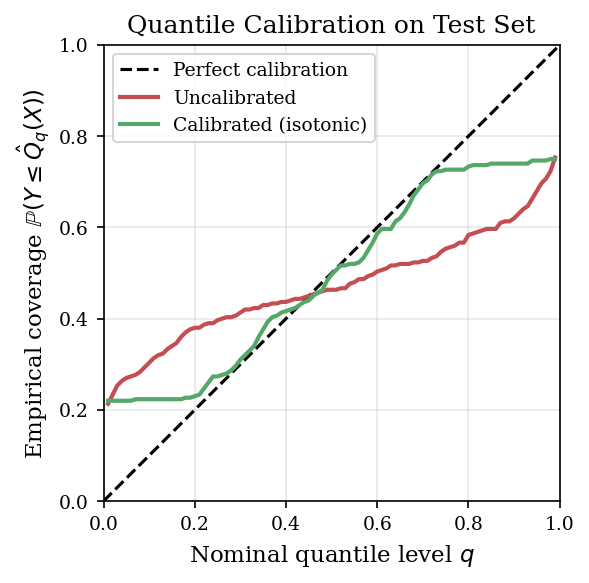
\includegraphics[width=0.65\textwidth]{figures/quantile_calibration.png}
\caption{Quantile calibration: diagonal = perfect; uncalibrated model deviates; isotonic calibration corrects.}
\label{fig:quantile_calibration}
\end{figure}

\Cref{fig:quantile_calibration} illustrates the distinction. A well-calibrated model produces quantiles such that when we predict the $q$-quantile $\hat{Q}_q(X)$, the fraction of held-out outcomes $Y \leq \hat{Q}_q(X)$ is approximately $q$. The diagonal represents this ideal. An uncalibrated model may deviate: for example, an overconfident model (underestimated variance) yields empirical coverage below the diagonal at high nominal levels. Post-hoc calibration methods such as isotonic regression can correct this by learning a monotone mapping from predicted to calibrated quantile levels on a validation set.

\subsection{Distribution-Free Coverage via Conformal Prediction}

Conformal prediction offers an alternative approach to uncertainty quantification by providing finite-sample, distribution-free coverage guarantees under minimal assumptions. Introduced by Shafer and Vovk \cite{shafer2008tutorial}, conformal prediction constructs prediction sets that contain the true outcome with a specified probability, provided the data are exchangeable. Crucially, these guarantees hold regardless of the correctness of the underlying predictive model.

Recent work has integrated conformal prediction with quantile regression to produce calibrated prediction intervals that adapt to heteroscedasticity in the data. Romano et al. \cite{romano2019conformalized} proposed conformalized quantile regression, which adjusts estimated conditional quantiles to ensure exact marginal coverage. This method preserves the flexibility of quantile regression while enforcing rigorous statistical guarantees, making it particularly attractive for safety-critical applications.

The primary limitation of conformal prediction methods is their inherent conservatism. Coverage guarantees are typically marginal rather than conditional, and the resulting prediction intervals may be wider than necessary for individual inputs. This trade-off between coverage guarantees and predictive sharpness reflects a fundamental tension in uncertainty quantification. Regardless, conformal prediction provides a robust and model-agnostic mechanism for uncertainty estimation, complementing calibration-based approaches and motivating hybrid methods that balance expressiveness, calibration, and statistical rigor.

\subsection{Proper Scoring Rules and Evaluation Metrics}

Evaluating probabilistic forecasts requires metrics that jointly assess both calibration and sharpness. Proper scoring rules provide a principled framework for this purpose by assigning a numerical score to a predicted distribution such that the expected score is minimized when the predictive distribution matches the true data-generating distribution. Gneiting and Raftery \cite{gneiting2007proper} formalized this framework and emphasized that calibration and sharpness must be considered together rather than as competing objectives.

Commonly used proper scoring rules include the logarithmic score, the continuous ranked probability score (CRPS), and interval-based scores. Unlike point-error metrics, proper scoring rules penalize both overconfident and overly diffuse predictions, making them well suited for comparing probabilistic models. As a result, they have become standard tools for evaluating probabilistic forecasts across a wide range of applications, including time series prediction and uncertainty-aware regression.

In the context of safety-critical forecasting, proper scoring rules provide an objective means of assessing whether probabilistic predictions are both reliable and informative. Their use complements calibration diagnostics and coverage-based guarantees, offering a unified evaluation framework for probabilistic regression models.

\section*{Synthesis and Implications}

Taken together, the literature reviewed in this chapter establishes what a surrogate of longitudinal train dynamics must provide and where existing approaches fall short. Classical longitudinal dynamics models supply well-understood physical structure, but their cost, concentrated in the stiff and nonlinear coupler interactions, keeps them out of optimization and control loops. Data-driven rail surrogates show that this cost can be reduced substantially, yet each is tied to something particular: a coupler position, a consist configuration, a track segment, or an operational context, and a change in that quantity requires retraining or configuration-specific adaptation data.

Sequence models and neural operators offer general machinery for learning dynamics, but both fix the size of their input in advance, so consist length, the quantity over which generalization is sought, becomes an architectural constant. Graph networks remove that constraint. Their structure matches the mechanics of a consist directly, with couplers as edges and the force balance as a node update, and the graph network simulator lineage shows that a learned fixed step can be stable over long rollouts and is not bound by the step-size limit of the scheme it replaces. Neural ODEs, the continuous-time alternative, face a documented difficulty on stiff systems, and a coupled vehicle chain is stiff by construction. What has not been done is to apply this machinery to the forward longitudinal dynamics of a coupled consist.

The probabilistic forecasting literature bears on a narrower question in this thesis than it would in a forecasting study. It establishes that expressive models do not produce reliable uncertainty estimates by default, and that calibration and coverage must be checked rather than assumed. Because the downstream use of the surrogate is control, uncertainty enters here as a coupler-force safety margin that the controller must respect, not as a calibrated distribution reported over every output, and it is evaluated in that role.

The gap this thesis addresses is therefore a surrogate that is train-agnostic by construction, imposes the physics it knows exactly rather than learning it, and is differentiable end to end so that it can serve as the model inside a fuel-optimal controller. \Cref{ch:problem} formulates that problem, and the surrogate itself is a graph network simulator on the consist's chain graph.
